\documentclass[aspectratio=169]{beamer}
\usepackage[utf8]{inputenc}
\usepackage{transparent}
\usepackage{hyperref}
\usepackage{pgf}
\usepackage{dsfont}
\usepackage{algorithm}
\usepackage{algorithmic}

% here comes my custom theme for university of Bamberg

\logo{\pgfputat{\pgfxy(-1.25,4.25)}{\pgfbox[center,base]{\transparent{0.7} 
\includegraphics[width=.15\textwidth]{uni_bamberg.png}}}}


\newcommand{\nologo}{\setbeamertemplate{logo}{}} % command to set the logo to nothing
\newcommand{\biglogo}{\setbeamertemplate{logo}{\pgfputat{\pgfxy(-2,4)}{\pgfbox[center,base]{ 
\includegraphics[width=.24\textwidth]{uni_bamberg.png}}}}} 

% theming and colors and stuff
\usetheme[progressbar=frametitle, block = fill]{metropolis}
\definecolor{uniblau}{RGB}{4, 66, 119} %#044277
\definecolor{niceorange}{RGB}{255, 128, 0} %#ff8000
\definecolor{nicegray}{RGB}{221, 239, 244} %#ddeff4
\setbeamercolor{palette primary}{bg=uniblau, fg=white}
\setbeamercolor{normal text}{fg=uniblau, bg=white}
\setbeamercolor{itemize item}{fg=niceorange}
\setbeamercolor{itemize subitem}{fg=niceorange}
\setbeamercolor{itemize subsubitem}{fg=niceorange}
\setbeamercolor{enumerate item}{fg=niceorange}
\setbeamercolor{enumerate subitem}{fg=niceorange}
\setbeamercolor{enumerate subsubitem}{fg=niceorange}
\setbeamercolor{block body}{bg=nicegray}
\setbeamercolor{block title}{bg=niceorange,fg=white}
\renewcommand\UrlFont{\color{niceorange}\rmfamily}

% own commands for highlighting
\newcommand{\pop}[1]{{\color{niceorange}\textbf{#1}}}

\def\ps@titlepage{\setbeamertemplate{footline}{}}
\makeatletter
\setbeamertemplate{frame footer}{\tiny{xAI-Proj-M - Model Engineering - B.Bony}}

% custom python style

%title page
\title{Model Engineering  -- Dropout Layers}
\subtitle{Explainable Machine Learning - Deep Learning Life Cycle}
\author{Jonas Amling \and Baptiste Bony \and Benedikt Marsiske}
\institute{University of Bamberg}
\date{\today} 

\begin{document}
% titleframe
{\biglogo
	\setbeamertemplate{footline}{} 
	\begin{frame}{}
		\titlepage
	\end{frame}
}

\begin{frame}{Table of contents}
	\tableofcontents
\end{frame}


{\nologo
\section{Research Question}
	\begin{frame}{Research Question and Introduction}
	Our main Model Engineering challenges:
	\begin{itemize}
		\item Accuracy performance
		\item Prevent overfitting for the model to be generalizable to new data
	\end{itemize}
	Research Question: \pop{Do dropout layers prevent overfitting and what's the ideal position for them in the model?} 
	\end{frame}

 
\section{Model Engineering Process}

    \begin{frame}{Dataset Overview}
        \begin{figure}
            \centering
            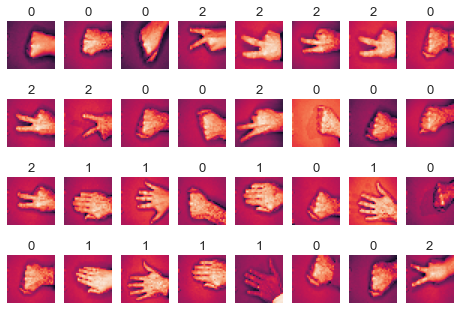
\includegraphics[width=0.5\textwidth]{img/green_background_dataset.png}
            \caption{Labeled Training Data from the Green Background Dataset}
        \end{figure}    
    \end{frame}

    
    \begin{frame}{Our Convolutional Neural Network}
        \begin{figure}
            \centering
            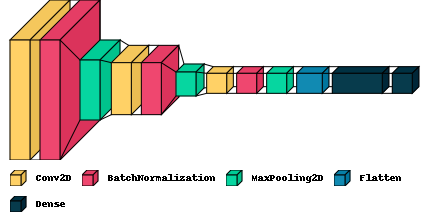
\includegraphics[width=0.6\textwidth]{img/model_without_dropout.png}
            \caption{Visualization of the Convolutional Neural Network without Dropout Layers}
        \end{figure}
    \end{frame}
    
    
    \begin{frame}{Problem Description : Overfitting}
        \begin{figure}
            \centering
            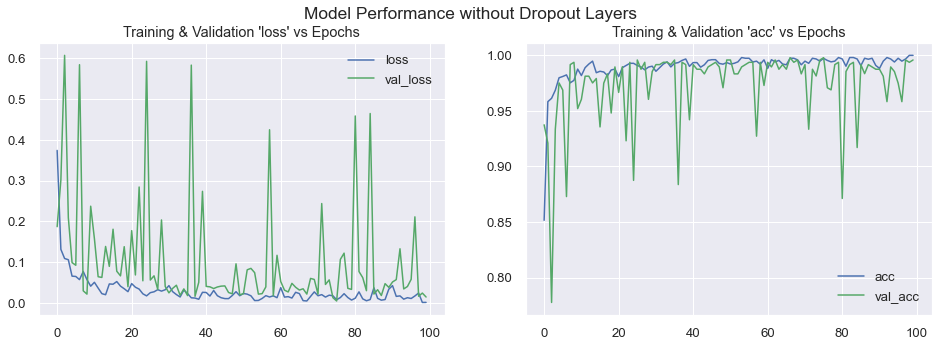
\includegraphics[width=0.8\textwidth]{img/plot_without_dropout.png}
            \caption{Model Performance without Dropout Layers}
        \end{figure}    
    \end{frame}

    \begin{frame}{Potential Solution: Dropout Layers}
        \begin{figure}
            \centering
            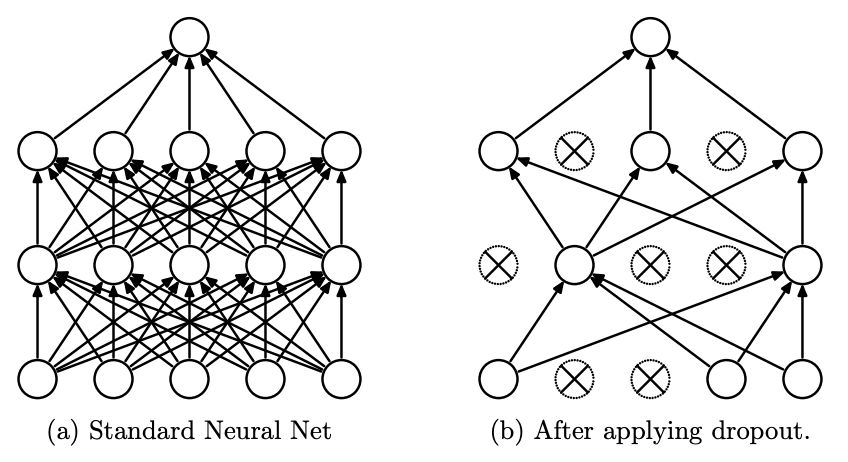
\includegraphics[width=0.6\textwidth]{img/dropout_schema.png}
            \caption{Scheme explaining the principle of Dropout Layers}
        \end{figure}    
    \end{frame}

    
    \begin{frame}{Our Convolutional Neural Network with Dropout Layers}
        \begin{figure}
            \centering
            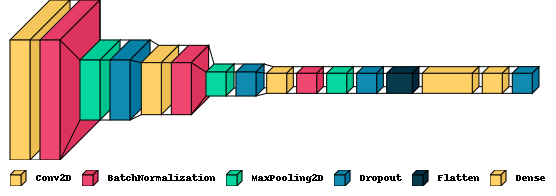
\includegraphics[width=0.8\textwidth]{img/model_with_dropout.png}
            \caption{Visualization of the Convolutional Neural Network with Dropout Layers}
        \end{figure}    
    \end{frame}
    
    \begin{frame}{Model Performance with Dropout}
        \begin{figure}
            \centering
            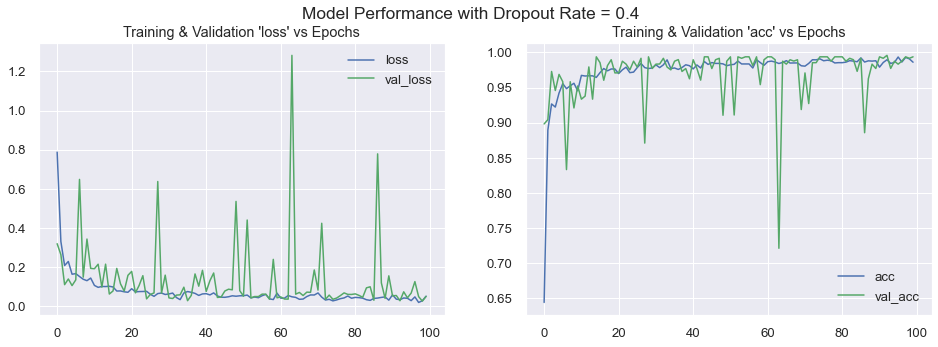
\includegraphics[width=0.8\textwidth]{img/plot_dropout_04.png}
            \caption{Model Performance with Dropout Rate = 0.4}
        \end{figure}    
    \end{frame}

    \begin{frame}{Model Performance with Dropout}
        \begin{figure}
            \centering
            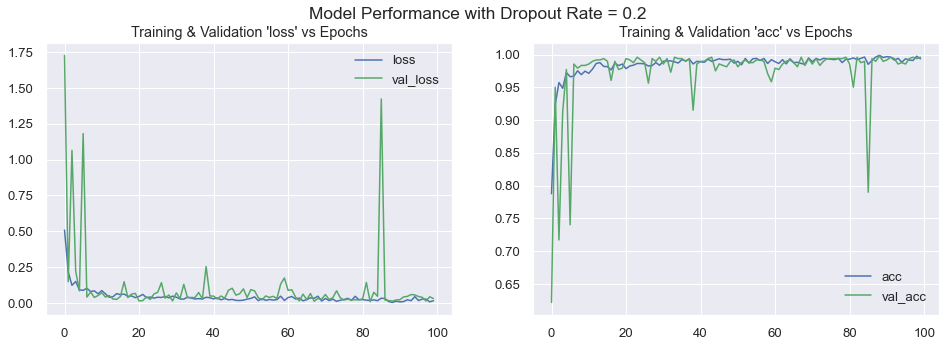
\includegraphics[width=0.8\textwidth]{img/plot_dropout_02.png}
            \caption{Model Performance with Dropout Rate = 0.2}
        \end{figure}    
    \end{frame}


    \begin{frame}{Dropout Limitations : Underfitting}
        \begin{figure}
            \centering
            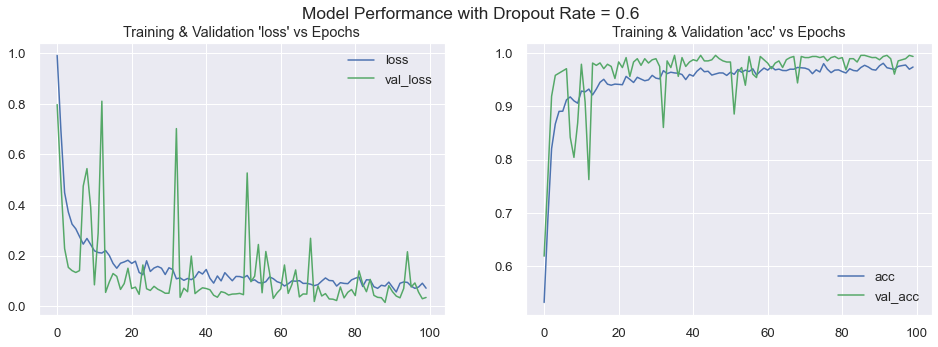
\includegraphics[width=0.8\textwidth]{img/plot_dropout_06.png}
            \caption{Model Performance with Dropout Rate = 0.6}
        \end{figure}    
    \end{frame}


\section{Looking back at Data Engineering}

    \begin{frame}{Research Question}
        A look back at the previous Research Question regarding Data Engineering
        
        \pop{Does removing the background during the image preprocessing phase benefit the image classification task at hand?}
    \end{frame}
    
    \begin{frame}{Raw Dataset}
        \begin{figure}
            \centering
            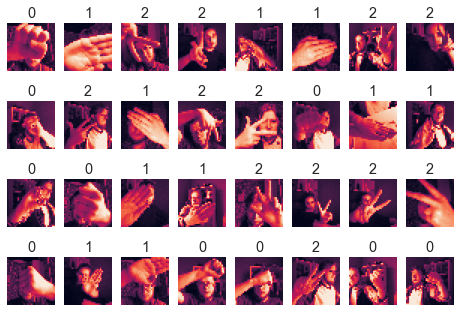
\includegraphics[width=0.5\textwidth]{img/webcam_dataset.png}
            \caption{Labeled Training Raw Data from the Webcam Dataset}
        \end{figure}    
    \end{frame}

    \begin{frame}{Model Performance without Preprocessing}
        \begin{figure}
            \centering
            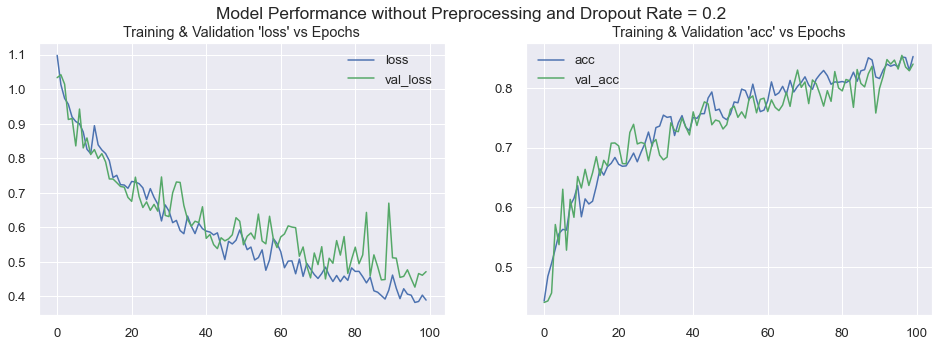
\includegraphics[width=0.8\textwidth]{img/plot_raw_02.png}
            \caption{Model Performance without Preprocessing \& Dropout Rate = 0.2}
        \end{figure}    
    \end{frame}   

    \begin{frame}{Model Performance without Preprocessing}
        \begin{figure}
            \centering
            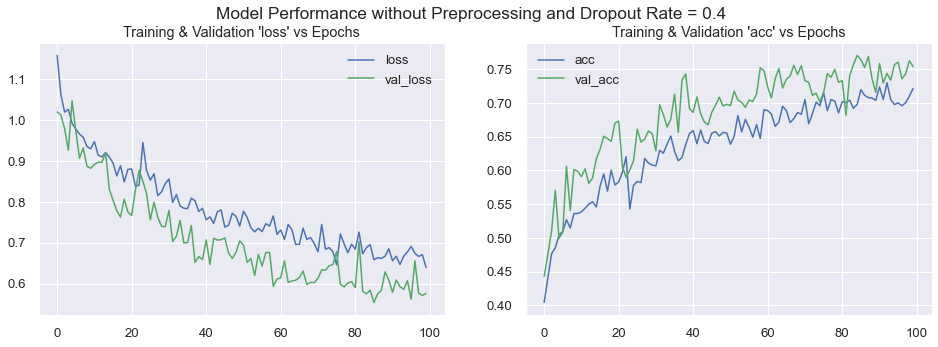
\includegraphics[width=0.8\textwidth]{img/plot_raw_04.png}
            \caption{Model Performance without Preprocessing \& Dropout Rate = 0.4}
        \end{figure}    
    \end{frame}
    
    \begin{frame}{Preprocessed Dataset}
        \begin{figure}
            \centering
            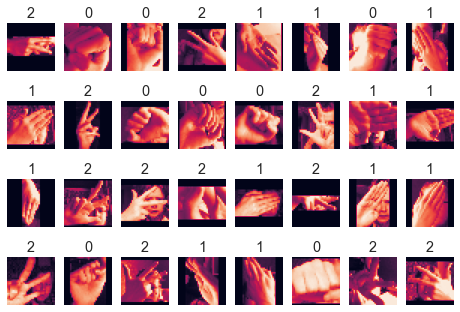
\includegraphics[width=0.5\textwidth]{img/webcam_dataset_preprocessed.png}
            \caption{Labeled Training Preprocessed Data from the Webcam Dataset}
        \end{figure}    
    \end{frame}

    \begin{frame}{Model Performance with Preprocessing}
        \begin{figure}
            \centering
            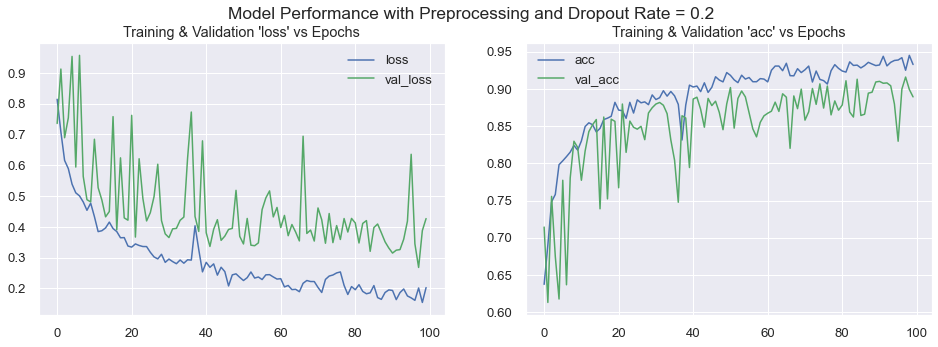
\includegraphics[width=0.8\textwidth]{img/plot_preprocessed_02.png}
            \caption{Model Performance with Preprocessing \& Dropout Rate = 0.2}
        \end{figure}    
    \end{frame}   

    \begin{frame}{Model Performance with Preprocessing}
        \begin{figure}
            \centering
            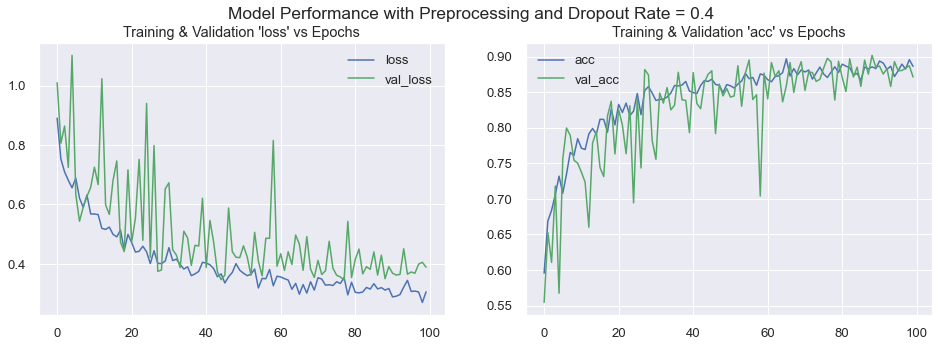
\includegraphics[width=0.8\textwidth]{img/plot_preprocessed_04.png}
            \caption{Model Performance with Preprocessing \& Dropout Rate = 0.4}
        \end{figure}    
    \end{frame}

\section{Further Considerations}

    \begin{frame}{Discussion}
        Issues we have not address yet :
	    \begin{itemize}
		      \item What influence does the optimizer have on the efficiency of the dropout?
		      \item Is it necessary to use batch normalization in addition to dropout?
            \item How about considering the number of epochs as a parameter and explore early stopping?
	    \end{itemize}
    \end{frame}

% finally our last stuff
\appendix
{\nologo
	\begin{frame}[standout]
		Thank you for your attention!
        \\
        Do you have any questions?
	\end{frame}
}
\end{document}